% =============================================================================
% LangGraph ile Production-Ready AI Agent Mimarisi
% Best Practices & Scaling Stratejileri
% =============================================================================
\documentclass[aspectratio=169, 11pt]{beamer}

% ---------- Tema ve Renk ----------
\usetheme{Madrid}
\usecolortheme{whale}

\definecolor{lgPrimary}{RGB}{30, 58, 138}      % Koyu mavi
\definecolor{lgSecondary}{RGB}{59, 130, 246}    % Açık mavi
\definecolor{lgAccent}{RGB}{16, 185, 129}       % Yeşil
\definecolor{lgWarn}{RGB}{245, 158, 11}         % Turuncu
\definecolor{lgDanger}{RGB}{239, 68, 68}        % Kırmızı
\definecolor{lgBg}{RGB}{241, 245, 249}          % Açık gri arka plan
\definecolor{lgDark}{RGB}{15, 23, 42}           % Koyu metin

\setbeamercolor{palette primary}{bg=lgPrimary, fg=white}
\setbeamercolor{palette secondary}{bg=lgSecondary, fg=white}
\setbeamercolor{palette tertiary}{bg=lgPrimary, fg=white}
\setbeamercolor{structure}{fg=lgPrimary}
\setbeamercolor{title}{fg=white, bg=lgPrimary}
\setbeamercolor{frametitle}{fg=white, bg=lgPrimary}
\setbeamercolor{block title}{bg=lgSecondary, fg=white}
\setbeamercolor{block body}{bg=lgBg, fg=lgDark}
\setbeamercolor{block title alerted}{bg=lgDanger, fg=white}
\setbeamercolor{block body alerted}{bg=lgBg, fg=lgDark}
\setbeamercolor{block title example}{bg=lgAccent, fg=white}
\setbeamercolor{block body example}{bg=lgBg, fg=lgDark}
\setbeamercolor{itemize item}{fg=lgSecondary}
\setbeamercolor{itemize subitem}{fg=lgAccent}

% ---------- Paketler ----------
\usepackage[utf8]{inputenc}
\usepackage[T1]{fontenc}
\usepackage{tikz}
\usetikzlibrary{
  shapes.geometric,
  arrows.meta,
  positioning,
  calc,
  fit,
  backgrounds,
  decorations.pathreplacing,
  shadows.blur,
  chains,
  matrix
}
\usepackage{fontawesome5}
\usepackage{booktabs}
\usepackage{array}
\usepackage{graphicx}
\usepackage{xcolor}

% ---------- TikZ Stilleri ----------
\tikzset{
  % Genel kutu stilleri
  basenode/.style={
    rounded corners=6pt,
    minimum height=1cm,
    minimum width=2.8cm,
    text centered,
    font=\small\bfseries,
    text=white,
    blur shadow={shadow blur steps=5, shadow xshift=0.5mm, shadow yshift=-0.5mm}
  },
  primarybox/.style={basenode, fill=lgPrimary},
  secondarybox/.style={basenode, fill=lgSecondary},
  accentbox/.style={basenode, fill=lgAccent},
  warnbox/.style={basenode, fill=lgWarn, text=lgDark},
  dangerbox/.style={basenode, fill=lgDanger},
  % Ok stilleri
  arrow/.style={-{Stealth[length=3mm]}, thick, color=lgPrimary},
  dasharrow/.style={-{Stealth[length=3mm]}, thick, dashed, color=lgSecondary},
  biarrow/.style={{Stealth[length=3mm]}-{Stealth[length=3mm]}, thick, color=lgPrimary},
  % Arka plan kutusu
  bgbox/.style={
    rounded corners=8pt,
    fill=lgBg,
    draw=lgSecondary!40,
    line width=0.5pt,
    inner sep=10pt
  },
  % Küçük etiket
  label node/.style={
    font=\tiny,
    fill=white,
    rounded corners=2pt,
    inner sep=2pt
  },
  % Database silindiri
  database/.style={
    cylinder,
    cylinder uses custom fill,
    cylinder body fill=lgPrimary!20,
    cylinder end fill=lgPrimary!40,
    shape border rotate=90,
    draw=lgPrimary,
    minimum height=1.2cm,
    minimum width=1.5cm,
    font=\small\bfseries,
    text=lgDark
  },
}

% ---------- Başlık Bilgileri ----------
\title[LangGraph Scaling]{LangGraph ile Production-Ready\\AI Agent Mimarisi}
\subtitle{Best Practices \& Scaling Stratejileri}
\author{Sistem Mimarisi Sunumu}
\date{\today}
\institute{}

% =============================================================================
\begin{document}

% --- Kapak ---
\begin{frame}[plain]
  \titlepage
\end{frame}

% --- İçindekiler ---
\begin{frame}{Ajanda}
  \tableofcontents
\end{frame}

% =============================================================================
\section{Problem Tanımı}
% =============================================================================

% --- Slide 1: Neden LangGraph? ---
\begin{frame}{Neden LangGraph?}
  \begin{columns}[T]
    \begin{column}{0.48\textwidth}
      \begin{alertblock}{\faExclamationTriangle\; Klasik LLM Çağrısı}
        \begin{itemize}
          \item Tek seferlik istek $\rightarrow$ yanıt
          \item State yönetimi yok
          \item Hata durumunda baştan başla
          \item İnsan müdahalesi mümkün değil
        \end{itemize}
      \end{alertblock}
    \end{column}
    \begin{column}{0.48\textwidth}
      \begin{exampleblock}{\faCheckCircle\; LangGraph Agent}
        \begin{itemize}
          \item Çok adımlı, döngüsel iş akışları
          \item Kalıcı state (checkpoint)
          \item Hata $\rightarrow$ kaldığı yerden devam
          \item Human-in-the-loop desteği
        \end{itemize}
      \end{exampleblock}
    \end{column}
  \end{columns}

  \vspace{0.5cm}
  \centering
  
\begin{tikzpicture}
    \node[primarybox, minimum width=10cm, minimum height=0.8cm] {
      \faLightbulb\; LangGraph = Durum Makinesi + LLM + Kalıcı Bellek + Araç Kullanımı
    };
  \end{tikzpicture}
\end{frame}

% --- Slide 2: Scaling Sorunu ---
\begin{frame}{Scaling Sorunu: Darboğaz Nerede?}
  \centering
  \begin{tikzpicture}[scale=0.9, transform shape]
    % Sol taraf: Bekleme yığını
    \node[dangerbox, minimum width=5cm, minimum height=0.7cm] (wait1) at (0, 2.5)
      {\%95 — LLM API Yanıt Bekleme};
    \node[warnbox, minimum width=5cm, minimum height=0.7cm] (wait2) at (0, 1.5)
      {\%3 — Veritabanı I/O};
    \node[accentbox, minimum width=5cm, minimum height=0.7cm] (wait3) at (0, 0.5)
      {\%2 — State Routing \& Parse};

    % Açıklama
    \node[right=1.2cm of wait1, text width=5cm, font=\small] (exp1) {
      \textbf{2--30 saniye} per LLM çağrısı\\
      Bir workflow $\approx$ 15--25 çağrı
    };
    \node[right=1.2cm of wait3, text width=5cm, font=\small] (exp2) {
      CPU eklemek sorunu \textbf{çözmez}\\
      $\Rightarrow$ I/O-bound problem
    };

    % Ok
    \draw[arrow] (wait1.east) -- (exp1.west);
    \draw[arrow] (wait3.east) -- (exp2.west);

    % Alt mesaj
    \node[primarybox, minimum width=12cm, minimum height=0.8cm] at (2, -0.8) {
      \faKey\; Gerçek Darboğaz = LLM API Rate Limit + Eşzamanlı İstek Yönetimi
    };
  \end{tikzpicture}
\end{frame}

% =============================================================================
\section{LangGraph Temel Kavramları}
% =============================================================================

% --- Slide 3: StateGraph Yapısı ---
\begin{frame}{LangGraph StateGraph Yapısı}
  \centering
  \begin{tikzpicture}[node distance=1.5cm and 2.5cm, scale=0.85, transform shape]
    % Nodes
    \node[accentbox] (start) {\faPlay\; START};
    \node[secondarybox, right=2cm of start] (plan) {\faCogs\; Planlama};
    \node[secondarybox, right=2cm of plan] (exec) {\faRocket\; Yürütme};
    \node[warnbox, below=1.2cm of exec] (review) {\faUserCheck\; İnsan Onayı};
    \node[secondarybox, right=2cm of exec] (synth) {\faFileAlt\; Sentez};
    \node[dangerbox, right=2cm of synth] (end) {\faStop\; END};

    % Edges
    \draw[arrow] (start) -- (plan);
    \draw[arrow] (plan) -- (exec);
    \draw[arrow] (exec) -- (synth);
    \draw[arrow] (synth) -- (end);

    % Conditional edge
    \draw[dasharrow] (exec) -- node[label node, right] {onay gerekli} (review);
    \draw[dasharrow] (review) -- node[label node, below, text width=2cm, align=center] {onaylandı} (synth);
    \draw[dasharrow, color=lgDanger] (review.west) -- +(-1,0) |- node[label node, above, pos=0.25] {reddedildi} (plan.south);

    % Checkpoint annotations
    \foreach \nd in {plan, exec, review, synth} {
      \node[above=0.15cm of \nd, font=\tiny\color{lgAccent}] {\faDatabase\; checkpoint};
    }

    % Legend
    \node[below=2cm of review, text width=10cm, align=center, font=\small] {
      \textcolor{lgPrimary}{\rule{0.8cm}{2pt}} Normal akış \quad
      \textcolor{lgSecondary}{- - -} Koşullu dal \quad
      \textcolor{lgAccent}{\faDatabase} Her adımda state kaydedilir
    };
  \end{tikzpicture}
\end{frame}

% --- Slide 4: Checkpoint & Thread ---
\begin{frame}{Checkpoint \& Thread Mekanizması}
  \centering
  \begin{tikzpicture}[scale=0.85, transform shape]
    % Timeline
    \draw[thick, lgPrimary] (0,0) -- (13,0);

    % Steps
    \foreach \x/\lab/\icon in {
      1/Adım 1/\faCogs,
      3.5/Adım 2/\faRocket,
      6/Adım 3/\faUserCheck,
      8.5/CRASH/\faBolt,
      11/Adım 3'/\faRedo
    } {
      \node[circle, fill=lgSecondary, text=white, minimum size=0.6cm, font=\tiny]
        (s\x) at (\x, 0) {\icon};
      \node[below=0.3cm of s\x, font=\scriptsize\bfseries] {\lab};
    }

    % Checkpoints above
    \foreach \x in {1, 3.5, 6} {
      \draw[lgAccent, thick] (\x, 0.4) -- (\x, 1.2);
      \node[fill=lgAccent, text=white, rounded corners=3pt, font=\tiny, minimum height=0.5cm]
        at (\x, 1.5) {\faDatabase\; CP};
    }

    % Crash indicator
    \node[fill=lgDanger, text=white, rounded corners=3pt, font=\tiny, minimum height=0.5cm]
      at (8.5, 1.5) {\faExclamationTriangle\; Crash};

    % Resume arrow
    \draw[arrow, lgAccent, very thick] (6, 1.5) to[out=30, in=150]
      node[above, font=\scriptsize, text=lgAccent] {Son checkpoint'ten devam}
      (11, 1.5);

    % Thread ID
    \node[primarybox, minimum width=13cm, minimum height=0.7cm] at (6.5, -1.5) {
      \faFingerprint\; thread\_id = Her kullanıcı/çalıştırma için benzersiz kimlik
    };

    % Açıklama kutuları
    \node[bgbox, text width=5.5cm, font=\scriptsize] at (3, -3.2) {
      \textbf{\textcolor{lgPrimary}{State kaydedilir:}}\\
      $\bullet$ Tüm düğüm çıktıları\\
      $\bullet$ Mevcut düğüm pozisyonu\\
      $\bullet$ Mesaj geçmişi
    };
    \node[bgbox, text width=5.5cm, font=\scriptsize] at (10, -3.2) {
      \textbf{\textcolor{lgAccent}{Resume mantığı:}}\\
      $\bullet$ Aynı thread\_id ile çağır\\
      $\bullet$ input = None gönder\\
      $\bullet$ Son checkpoint'ten başlar
    };
  \end{tikzpicture}
\end{frame}

% =============================================================================
\section{Checkpointer Seçimi}
% =============================================================================

% --- Slide 5: Checkpointer Karşılaştırma ---
\begin{frame}{Checkpointer Seçimi}
  \centering
  \begin{tikzpicture}[scale=0.8, transform shape]
    % Headers
    \node[primarybox, minimum width=3.2cm] (h1) at (0, 4) {MemorySaver};
    \node[primarybox, minimum width=3.2cm] (h2) at (4.5, 4) {PostgresSaver};
    \node[primarybox, minimum width=3.2cm] (h3) at (9, 4) {RedisSaver};

    % Satırlar
    \def\rows{
      {Kalıcılık/Yok (RAM)/Disk-backed/RAM + Persist},
      {Restart Dayanıklılığı/\faTimesCircle\; Kaybolur/\faCheckCircle\; Korunur/\faCheckCircle\; Korunur},
      {Çoklu Worker/\faTimesCircle\; Tek process/\faCheckCircle\; Paylaşımlı/\faCheckCircle\; Dağıtık},
      {Hız/\faBolt\; En hızlı/\faClock\; Orta/\faBolt\; Çok hızlı},
      {Sorgulanabilirlik/Sınırlı/SQL + JSONB/RediSearch},
      {Kullanım Alanı/Geliştirme/\faCheckCircle\; Production/Yüksek throughput}
    }

    \foreach [count=\i] \row in \rows {
      \pgfmathsetmacro{\y}{4 - \i * 0.9}
      % Parse row
      \foreach [count=\j] \cell in \row {
        \pgfmathsetmacro{\x}{(\j - 1) * 4.5 - 4.5}
        \ifnum\j=1
          \node[font=\scriptsize\bfseries, text=lgDark, text width=2.8cm, align=right]
            at (\x, \y) {\cell};
        \else
          \pgfmathsetmacro{\xx}{(\j - 2) * 4.5}
          \node[bgbox, font=\scriptsize, text width=2.8cm, align=center, inner sep=4pt, minimum height=0.65cm]
            at (\xx, \y) {\cell};
        \fi
      }
    }

    % Recommendation arrow
    \node[accentbox, minimum width=4cm, minimum height=0.7cm] at (4.5, -2.5) {
      \faThumbsUp\; Production için PostgresSaver önerilir
    };

    \draw[arrow, lgAccent, very thick] (4.5, -2.1) -- (h2.south);
  \end{tikzpicture}
\end{frame}

% =============================================================================
\section{Durability Modları}
% =============================================================================

% --- Slide 6: Durability Modları ---
\begin{frame}{LangGraph Durability Modları (v0.6+)}
  \centering
  \begin{tikzpicture}[scale=0.85, transform shape]
    % SYNC
    \node[primarybox, minimum width=2.2cm] (sync_t) at (0, 3.5) {\texttt{sync}};
    \foreach \x/\lab in {0/A, 1.5/CP, 3/B, 4.5/CP, 6/C, 7.5/CP} {
      \ifnum\x=1 \node[fill=lgAccent, circle, minimum size=0.4cm, inner sep=0pt, font=\tiny, text=white] (sync\x) at (\x, 2.5) {\faDatabase};
      \else\ifnum\x=4 \node[fill=lgAccent, circle, minimum size=0.4cm, inner sep=0pt, font=\tiny, text=white] (sync\x) at (\x, 2.5) {\faDatabase};
      \else\ifnum\x=7 \node[fill=lgAccent, circle, minimum size=0.4cm, inner sep=0pt, font=\tiny, text=white] (sync\x) at (\x, 2.5) {\faDatabase};
      \else \node[fill=lgSecondary, rounded corners=3pt, minimum size=0.4cm, inner sep=0pt, font=\tiny, text=white] (sync\x) at (\x, 2.5) {\lab};
      \fi\fi\fi
    }
    \draw[thick, lgPrimary] (0, 2.5) -- (7.5, 2.5);
    \node[right, font=\scriptsize, text width=4cm] at (8.2, 2.5) {
      Her adımdan \textbf{önce} yazar\\
      \textcolor{lgDanger}{En yavaş} ama \textcolor{lgAccent}{en güvenli}
    };

    % ASYNC
    \node[secondarybox, minimum width=2.2cm] (async_t) at (0, 1.2) {\texttt{async}};
    \draw[thick, lgSecondary] (0, 0.2) -- (7.5, 0.2);
    \foreach \x/\lab in {0/A, 3/B, 6/C} {
      \node[fill=lgSecondary, rounded corners=3pt, minimum size=0.4cm, inner sep=0pt, font=\tiny, text=white] at (\x, 0.2) {\lab};
    }
    \foreach \x in {1.2, 4.2, 7.2} {
      \node[fill=lgAccent!60, circle, minimum size=0.35cm, inner sep=0pt, font=\tiny, text=white] at (\x, -0.3) {\faDatabase};
      \draw[dasharrow, lgAccent!60, thin] (\x - 1.2, 0.2) -- (\x, -0.3);
    }
    \node[right, font=\scriptsize, text width=4cm] at (8.2, 0) {
      Paralel olarak arka planda yazar\\
      \textcolor{lgWarn}{Hızlı}, \%99.9 güvenli
    };

    % EXIT
    \node[warnbox, minimum width=2.2cm] (exit_t) at (0, -1.5) {\texttt{exit}};
    \draw[thick, lgWarn] (0, -2.5) -- (7.5, -2.5);
    \foreach \x/\lab in {0/A, 3/B, 6/C} {
      \node[fill=lgWarn, rounded corners=3pt, minimum size=0.4cm, inner sep=0pt, font=\tiny, text=lgDark] at (\x, -2.5) {\lab};
    }
    \node[fill=lgAccent, circle, minimum size=0.4cm, inner sep=0pt, font=\tiny, text=white] at (7.5, -2.5) {\faDatabase};
    \node[right, font=\scriptsize, text width=4cm] at (8.2, -2.5) {
      Sadece \textbf{bitişte} yazar\\
      \textcolor{lgAccent}{En hızlı}, crash = baştan
    };

    % Recommendation
    \node[bgbox, text width=12cm, align=center, font=\small] at (4, -4) {
      \faLightbulb\; \textbf{Öneri:} Çoğu production sistemi için \texttt{async} $\mid$
      Finansal işlemler için \texttt{sync} $\mid$
      Batch işler için \texttt{exit}
    };
  \end{tikzpicture}
\end{frame}

% =============================================================================
\section{Scaling Mimarisi}
% =============================================================================

% --- Slide 7: Monolith vs Queue ---
\begin{frame}{Evrim: Monolith $\rightarrow$ Queue Mimarisi}
  \begin{columns}[T]
    \begin{column}{0.45\textwidth}
      \centering
      \textbf{\textcolor{lgDanger}{\faTimesCircle\; Monolith (Yanlış)}}
      \vspace{0.3cm}
      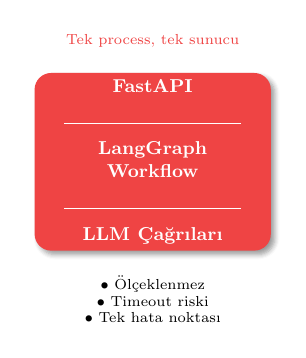
\begin{tikzpicture}[scale=0.75, transform shape]
        \node[dangerbox, minimum width=4cm, minimum height=3cm, align=center] (mono) {
          FastAPI\\[4pt]
          \rule{3cm}{0.4pt}\\[4pt]
          LangGraph\\
          Workflow\\[4pt]
          \rule{3cm}{0.4pt}\\[4pt]
          LLM Çağrıları
        };
        \node[above=0.3cm of mono, font=\scriptsize\color{lgDanger}] {
          Tek process, tek sunucu
        };
        \node[below=0.3cm of mono, font=\scriptsize, text width=4cm, align=center] {
          $\bullet$ Ölçeklenmez\\
          $\bullet$ Timeout riski\\
          $\bullet$ Tek hata noktası
        };
      \end{tikzpicture}
    \end{column}
    \begin{column}{0.08\textwidth}
      \centering
      \vspace{2cm}
      {\Huge\textcolor{lgAccent}{$\Rightarrow$}}
    \end{column}
    \begin{column}{0.45\textwidth}
      \centering
      \textbf{\textcolor{lgAccent}{\faCheckCircle\; Queue Mimarisi (Doğru)}}
      \vspace{0.3cm}
      \begin{tikzpicture}[scale=0.75, transform shape]
        \node[accentbox, minimum width=3.5cm] (api) at (0, 2) {\faServer\; API Katmanı};
        \node[warnbox, minimum width=3.5cm] (queue) at (0, 0.5) {\faStream\; Redis Queue};
        \node[secondarybox, minimum width=1.5cm] (w1) at (-1.5, -1.2) {\faCog\; W1};
        \node[secondarybox, minimum width=1.5cm] (w2) at (0, -1.2) {\faCog\; W2};
        \node[secondarybox, minimum width=1.5cm] (w3) at (1.5, -1.2) {\faCog\; W3};
        \node[database] (db) at (0, -3) {PG};

        \draw[arrow] (api) -- (queue);
        \draw[arrow] (queue) -- (w1);
        \draw[arrow] (queue) -- (w2);
        \draw[arrow] (queue) -- (w3);
        \draw[arrow] (w1) -- (db);
        \draw[arrow] (w2) -- (db);
        \draw[arrow] (w3) -- (db);

        \node[below=0.1cm of db, font=\scriptsize, text width=4cm, align=center] {
          $\bullet$ Yatay ölçeklenme\\
          $\bullet$ Worker bağımsız\\
          $\bullet$ Hata izolasyonu
        };
      \end{tikzpicture}
    \end{column}
  \end{columns}
\end{frame}

% --- Slide 8: Full Architecture ---
\begin{frame}{Production Mimarisi (100K+ Kullanıcı)}
  \centering
  \begin{tikzpicture}[scale=0.7, transform shape, node distance=0.8cm]
    % Kullanıcılar
    \node[font=\Large] (users) at (0, 5) {\faUsers\; \faUsers\; \faUsers};
    \node[above=0.1cm of users, font=\scriptsize\bfseries] {100K+ Kullanıcı};

    % Load Balancer
    \node[primarybox, minimum width=6cm] (lb) at (0, 3.5) {\faBalanceScale\; Load Balancer (Nginx / ALB)};
    \draw[arrow] (users) -- (lb);

    % API Pods
    \node[secondarybox, minimum width=1.8cm, minimum height=0.7cm, font=\tiny\bfseries] (api1) at (-3, 2) {API Pod 1};
    \node[secondarybox, minimum width=1.8cm, minimum height=0.7cm, font=\tiny\bfseries] (api2) at (-1, 2) {API Pod 2};
    \node[secondarybox, minimum width=1.8cm, minimum height=0.7cm, font=\tiny\bfseries] (api3) at (1, 2) {API Pod 3};
    \node[secondarybox, minimum width=1.8cm, minimum height=0.7cm, font=\tiny\bfseries] (api4) at (3, 2) {API Pod N};
    \draw[arrow] (lb) -- (api1);
    \draw[arrow] (lb) -- (api2);
    \draw[arrow] (lb) -- (api3);
    \draw[arrow] (lb) -- (api4);

    % HPA label
    \node[font=\tiny\color{lgAccent}, right=0.2cm of api4] {HPA: CPU \textgreater{}70\%};

    % Redis
    \node[warnbox, minimum width=6cm] (redis) at (0, 0.5) {\faStream\; Redis (Task Queue + Rate Limiter)};
    \draw[arrow] (api1.south) -- ++(0,-0.3) -| ([xshift=-1.5cm]redis.north);
    \draw[arrow] (api2.south) -- (redis.north -| api2);
    \draw[arrow] (api3.south) -- (redis.north -| api3);
    \draw[arrow] (api4.south) -- ++(0,-0.3) -| ([xshift=1.5cm]redis.north);

    % Workers
    \node[accentbox, minimum width=1.5cm, minimum height=0.7cm, font=\tiny\bfseries] (w1) at (-4, -1.3) {Worker 1};
    \node[accentbox, minimum width=1.5cm, minimum height=0.7cm, font=\tiny\bfseries] (w2) at (-2, -1.3) {Worker 2};
    \node[accentbox, minimum width=1.5cm, minimum height=0.7cm, font=\tiny\bfseries] (w3) at (0, -1.3) {Worker 3};
    \node[accentbox, minimum width=1.5cm, minimum height=0.7cm, font=\tiny\bfseries] (w4) at (2, -1.3) {Worker N};
    \draw[arrow] (redis) -- (w1);
    \draw[arrow] (redis) -- (w2);
    \draw[arrow] (redis) -- (w3);
    \draw[arrow] (redis) -- (w4);

    % HPA label workers
    \node[font=\tiny\color{lgAccent}, right=0.2cm of w4] {HPA: Queue depth \textgreater{}10};

    % İçerik detayı
    \begin{scope}[on background layer]
      \node[bgbox, fit=(w1)(w4), inner sep=8pt, label={[font=\tiny\color{lgPrimary}]below:LangGraph + Checkpoint + Fallback + Tracing}] {};
    \end{scope}

    % PostgreSQL
    \node[database, minimum width=2cm, minimum height=1.5cm] (pg) at (-2, -3.5) {PostgreSQL};
    \node[font=\tiny, below=0.05cm of pg, text width=2.5cm, align=center] {Checkpoints\\Threads\\State};

    % LLM Providers
    \node[primarybox, minimum width=3cm] (llm) at (3, -3.5) {\faRobot\; LLM Providers};
    \node[font=\tiny, below=0.05cm of llm, text width=3cm, align=center] {OpenAI $|$ Anthropic $|$ Fallback};

    % Connections to PG and LLM
    \draw[arrow] (w1) -- (pg);
    \draw[arrow] (w2) -- (pg);
    \draw[arrow] (w3) -- (pg);
    \draw[arrow] (w3) -- (llm);
    \draw[arrow] (w4) -- (llm);

    % LangSmith
    \node[primarybox, minimum width=4cm, fill=lgPrimary!70] (ls) at (7, 0.5) {\faChartLine\; LangSmith};
    \node[font=\tiny, below=0.05cm of ls, text width=3cm, align=center] {Traces, Dashboards\\Alerts, Cost Tracking};
    \draw[dasharrow, thin] (w4.east) -- ++(0.5, 0) |- (ls.west);
  \end{tikzpicture}
\end{frame}

% =============================================================================
\section{LLM Rate Limit Stratejisi}
% =============================================================================

% --- Slide 9: Rate Limit ---
\begin{frame}{LLM Rate Limit \& Fallback Stratejisi}
  \centering
  \begin{tikzpicture}[scale=0.8, transform shape]
    % İstek akışı
    \node[secondarybox, minimum width=2.5cm] (req) at (0, 3) {\faComment\; İstek};

    % Rate Limiter
    \node[warnbox, minimum width=3.5cm, minimum height=1.2cm] (rl) at (0, 1) {
      \faShieldAlt\; Rate Limiter\\
      \tiny (Redis Token Bucket)
    };
    \draw[arrow] (req) -- (rl);

    % Decision
    \node[diamond, fill=lgSecondary, text=white, minimum size=0.8cm, font=\tiny, inner sep=1pt]
      (dec) at (0, -0.8) {Limit?};
    \draw[arrow] (rl) -- (dec);

    % OK path
    \node[accentbox, minimum width=2.5cm] (p1) at (-4, -2.5) {\faRobot\; Primary LLM};
    \draw[arrow, lgAccent] (dec) -| node[label node, pos=0.25, above] {OK} (p1);

    % Wait path
    \node[dangerbox, minimum width=2.5cm] (wait) at (4, -0.8) {\faClock\; Bekle + Retry};
    \draw[arrow, lgDanger] (dec) -- node[label node, above] {Limit aşıldı} (wait);
    \draw[arrow, lgDanger] (wait) |- ([yshift=0.5cm]rl.east) -- (rl.east);

    % Fallback chain
    \node[diamond, fill=lgSecondary, text=white, minimum size=0.8cm, font=\tiny, inner sep=1pt]
      (dec2) at (-4, -4.2) {Hata?};
    \draw[arrow] (p1) -- (dec2);

    \node[warnbox, minimum width=2.5cm] (f1) at (0, -4.2) {\faRobot\; Fallback \#1};
    \draw[arrow] (dec2) -- node[label node, above] {429 / Timeout} (f1);

    \node[dangerbox, minimum width=2.5cm] (f2) at (4, -4.2) {\faRobot\; Fallback \#2};
    \draw[arrow] (f1) -- node[label node, above] {Hata} (f2);

    % Success paths
    \node[accentbox, minimum width=3cm] (ok) at (0, -6) {\faCheckCircle\; Yanıt};
    \draw[arrow, lgAccent] (dec2) |- node[label node, pos=0.25, left] {Başarılı} (ok);
    \draw[arrow, lgAccent] (f1) -- (ok);
    \draw[arrow, lgAccent] (f2) |- (ok);

    % Provider examples
    \node[bgbox, font=\tiny, text width=3cm, align=center] at (-4, -5.8) {
      \textbf{Primary:} Claude Sonnet\\
      \textbf{Fallback 1:} GPT-4o\\
      \textbf{Fallback 2:} GPT-4o-mini
    };
  \end{tikzpicture}
\end{frame}

% =============================================================================
\section{Double Texting Stratejileri}
% =============================================================================

% --- Slide 10: Double Texting ---
\begin{frame}{Double Texting: Eşzamanlı Mesaj Yönetimi}
  \small
  \begin{columns}[T]
    \begin{column}{0.48\textwidth}
      \begin{block}{\faStream\; Enqueue (Sıraya Al)}
        \centering
        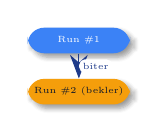
\begin{tikzpicture}[scale=0.65, transform shape]
          \node[secondarybox, minimum width=2cm, minimum height=0.5cm, font=\tiny] (r1) at (0,1) {Run \#1};
          \node[warnbox, minimum width=2cm, minimum height=0.5cm, font=\tiny] (r2) at (0,0) {Run \#2 (bekler)};
          \draw[arrow, thin] (r1) -- node[label node, right] {biter} (r2);
        \end{tikzpicture}
        \\[2pt]
        {\scriptsize Yeni mesaj kuyruğa eklenir, sırasıyla işlenir.}
      \end{block}
      \vspace{0.3cm}
      \begin{block}{\faBan\; Reject (Reddet)}
        \centering
        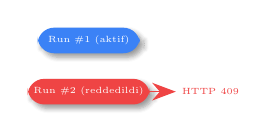
\begin{tikzpicture}[scale=0.65, transform shape]
          \node[secondarybox, minimum width=2cm, minimum height=0.5cm, font=\tiny] (r1) at (0,1) {Run \#1 (aktif)};
          \node[dangerbox, minimum width=2cm, minimum height=0.5cm, font=\tiny] (r2) at (0,0) {Run \#2 (reddedildi)};
          \draw[arrow, lgDanger, thin] (r2.east) -- ++(0.5,0) node[right, font=\tiny] {HTTP 409};
        \end{tikzpicture}
        \\[2pt]
        {\scriptsize Mevcut çalışma varken yeni istek reddedilir.}
      \end{block}
    \end{column}
    \begin{column}{0.48\textwidth}
      \begin{block}{\faHandPaper\; Interrupt (Durdur)}
        \centering
        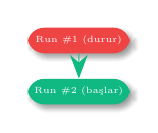
\begin{tikzpicture}[scale=0.65, transform shape]
          \node[dangerbox, minimum width=2cm, minimum height=0.5cm, font=\tiny] (r1) at (0,1) {Run \#1 (durur)};
          \node[accentbox, minimum width=2cm, minimum height=0.5cm, font=\tiny] (r2) at (0,0) {Run \#2 (başlar)};
          \draw[arrow, lgAccent, thin] (r1) -- (r2);
        \end{tikzpicture}
        \\[2pt]
        {\scriptsize Mevcut çalışma durdurulur, yenisi hemen başlar.}
      \end{block}
      \vspace{0.3cm}
      \begin{block}{\faUndo\; Rollback (Geri Al)}
        \centering
        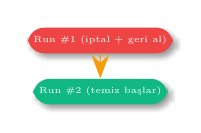
\begin{tikzpicture}[scale=0.65, transform shape]
          \node[dangerbox, minimum width=2cm, minimum height=0.5cm, font=\tiny] (r1) at (0,1) {Run \#1 (iptal + geri al)};
          \node[accentbox, minimum width=2cm, minimum height=0.5cm, font=\tiny] (r2) at (0,0) {Run \#2 (temiz başlar)};
          \draw[arrow, lgWarn, thin] (r1) -- (r2);
        \end{tikzpicture}
        \\[2pt]
        {\scriptsize Mevcut çalışma geri alınır, state sıfırlanarak yenisi başlar.}
      \end{block}
    \end{column}
  \end{columns}

  \vspace{0.3cm}
  \centering
  
\begin{tikzpicture}
    \node[primarybox, minimum width=10cm, minimum height=0.7cm, font=\small] {
      \faLightbulb\; Chatbot $\rightarrow$ Interrupt \quad\quad Batch İşlem $\rightarrow$ Enqueue \quad\quad Ödeme $\rightarrow$ Reject
    };
  \end{tikzpicture}
\end{frame}

% =============================================================================
\section{Auto-Scaling Kuralları}
% =============================================================================

% --- Slide 11: Auto-Scaling ---
\begin{frame}{Kubernetes Auto-Scaling Kuralları}
  \centering
  \begin{tikzpicture}[scale=0.8, transform shape]
    % Metrik kutuları
    \node[secondarybox, minimum width=4cm, minimum height=1.2cm, align=center] (m1) at (-4.5, 2) {
      \faMicrochip\; API Pod CPU\\
      \tiny Threshold: \textgreater{}70\%
    };
    \node[warnbox, minimum width=4cm, minimum height=1.2cm, align=center] (m2) at (0, 2) {
      \faStream\; Redis Queue Depth\\
      \tiny Threshold: \textgreater{}10 / worker
    };
    \node[accentbox, minimum width=4cm, minimum height=1.2cm, align=center] (m3) at (4.5, 2) {
      \faDatabase\; PG Connections\\
      \tiny Threshold: \textgreater{}80\% pool
    };
    \node[dangerbox, minimum width=4cm, minimum height=1.2cm, align=center] (m4) at (-2.25, -0.3) {
      \faExclamationTriangle\; LLM 429 Rate\\
      \tiny Threshold: \textgreater{}5\%
    };
    \node[primarybox, minimum width=4cm, minimum height=1.2cm, align=center] (m5) at (2.25, -0.3) {
      \faClock\; Workflow Latency\\
      \tiny Threshold: P99 \textgreater{} 60s
    };

    % Aksiyonlar
    \draw[arrow] (m1.south) -- ++(0, -0.4) node[below, font=\scriptsize, text=lgDark, text width=3.5cm, align=center] {
      $\Rightarrow$ API pod ekle\\(HPA autoscale)
    };
    \draw[arrow] (m2.south) -- ++(0, -0.4) node[below, font=\scriptsize, text=lgDark, text width=3.5cm, align=center] {
      $\Rightarrow$ Worker pod ekle\\(KEDA / Custom HPA)
    };
    \draw[arrow] (m3.south) -- ++(0, -0.4) node[below, font=\scriptsize, text=lgDark, text width=3.5cm, align=center] {
      $\Rightarrow$ PgBouncer scale\\+ Read replica
    };
    \draw[arrow] (m4.south) -- ++(0, -0.5) node[below, font=\scriptsize, text=lgDark, text width=3.5cm, align=center] {
      $\Rightarrow$ Fallback provider\\aktifleştir
    };
    \draw[arrow] (m5.south) -- ++(0, -0.5) node[below, font=\scriptsize, text=lgDark, text width=3.5cm, align=center] {
      $\Rightarrow$ Workflow optimize\\veya worker ekle
    };

    % Cool-down note
    \node[bgbox, text width=10cm, align=center, font=\scriptsize] at (0, -3.5) {
      \faInfoCircle\; \textbf{Scale-down cool-down:} 30 dakika $\mid$
      Ani düşüşlerde pod'lar hemen silinmez, thrashing önlenir
    };
  \end{tikzpicture}
\end{frame}

% =============================================================================
\section{Observability}
% =============================================================================

% --- Slide 12: LangSmith Observability ---
\begin{frame}{LangSmith ile End-to-End Observability}
  \centering
  \begin{tikzpicture}[scale=0.8, transform shape]
    % Merkez: LangSmith
    \node[primarybox, minimum width=3.5cm, minimum height=1.5cm, align=center]
      (ls) at (0, 0) {\faChartLine\; \textbf{LangSmith}\\[2pt]\tiny Async Collector\\Sıfır Latency};

    % Veri kaynakları (sol)
    \node[secondarybox, minimum width=2.8cm] (src1) at (-5.5, 2) {\faCogs\; LLM Çağrıları};
    \node[accentbox, minimum width=2.8cm] (src2) at (-5.5, 0.5) {\faWrench\; Tool Çağrıları};
    \node[warnbox, minimum width=2.8cm] (src3) at (-5.5, -1) {\faProjectDiagram\; Graph Adımları};
    \node[dangerbox, minimum width=2.8cm] (src4) at (-5.5, -2.5) {\faExclamationTriangle\; Hatalar};

    \draw[arrow] (src1) -- (ls);
    \draw[arrow] (src2) -- (ls);
    \draw[arrow] (src3) -- (ls);
    \draw[arrow] (src4) -- (ls);

    % Çıktılar (sağ)
    \node[secondarybox, minimum width=3cm] (out1) at (5.5, 2.5) {\faTachometerAlt\; P50/P99 Latency};
    \node[accentbox, minimum width=3cm] (out2) at (5.5, 1) {\faCoins\; Token \& Maliyet};
    \node[warnbox, minimum width=3cm] (out3) at (5.5, -0.5) {\faBell\; Alertler};
    \node[primarybox, minimum width=3cm] (out4) at (5.5, -2) {\faSearch\; Trace Arama};

    \draw[arrow] (ls) -- (out1);
    \draw[arrow] (ls) -- (out2);
    \draw[arrow] (ls) -- (out3);
    \draw[arrow] (ls) -- (out4);

    % Alt not
    \node[bgbox, text width=12cm, align=center, font=\small] at (0, -4) {
      \faShieldAlt\; LangSmith çökse bile uygulamanız \textbf{etkilenmez} $\mid$
      Tüm trace'ler \textbf{async} gönderilir $\mid$
      \textbf{OpenTelemetry} uyumlu
    };
  \end{tikzpicture}
\end{frame}

% =============================================================================
\section{Deployment Seçenekleri}
% =============================================================================

% --- Slide 13: Deployment ---
\begin{frame}{LangGraph Deployment Seçenekleri}
  \centering
  \begin{tikzpicture}[scale=0.75, transform shape]
    % 4 kolon
    \def\colw{3.2cm}

    % Cloud SaaS
    \node[primarybox, minimum width=\colw, minimum height=1cm] (c1) at (-5.2, 3) {
      \faCloud\; Cloud SaaS
    };
    \node[bgbox, text width=2.8cm, align=left, font=\tiny] (d1) at (-5.2, 0.8) {
      $\bullet$ Tam yönetilen\\
      $\bullet$ 1-click deploy\\
      $\bullet$ GitHub entegrasyonu\\
      $\bullet$ 10 container'a kadar\\[3pt]
      \textbf{İçin:} Hızlı başlangıç,\\küçük-orta takımlar
    };

    % BYOC
    \node[secondarybox, minimum width=\colw, minimum height=1cm] (c2) at (-1.7, 3) {
      \faServer\; BYOC
    };
    \node[bgbox, text width=2.8cm, align=left, font=\tiny] (d2) at (-1.7, 0.8) {
      $\bullet$ Sizin VPC'nizde\\
      $\bullet$ AWS ECS + Terraform\\
      $\bullet$ Veri dışarı çıkmaz\\
      $\bullet$ Control plane yönetilen\\[3pt]
      \textbf{İçin:} Uyumluluk,\\veri egemenliği
    };

    % Self-Hosted Lite
    \node[accentbox, minimum width=\colw, minimum height=1cm] (c3) at (1.8, 3) {
      \faDocker\; Self-Hosted Lite
    };
    \node[bgbox, text width=2.8cm, align=left, font=\tiny] (d3) at (1.8, 0.8) {
      $\bullet$ Ücretsiz (1M node)\\
      $\bullet$ Helm chart mevcut\\
      $\bullet$ Siz yönetirsiniz\\
      $\bullet$ PG + Redis + Docker\\[3pt]
      \textbf{İçin:} Geliştirme,\\küçük ölçek
    };

    % Self-Hosted Enterprise
    \node[warnbox, minimum width=\colw, minimum height=1cm] (c4) at (5.3, 3) {
      \faBuilding\; Enterprise
    };
    \node[bgbox, text width=2.8cm, align=left, font=\tiny] (d4) at (5.3, 0.8) {
      $\bullet$ Tam özellik seti\\
      $\bullet$ Kendi altyapınız\\
      $\bullet$ Kubernetes native\\
      $\bullet$ Lisanslı\\[3pt]
      \textbf{İçin:} Büyük kurumlar,\\maksimum kontrol
    };

    % Scale arrow
    \draw[{Stealth[length=4mm]}-{Stealth[length=4mm]}, very thick, lgPrimary]
      (-6.5, -1) -- (6.5, -1)
      node[midway, below, font=\small\bfseries] {Kontrol $\longleftrightarrow$ Kolaylık};
    \node[font=\scriptsize\color{lgAccent}] at (-5.5, -1.6) {Daha kolay};
    \node[font=\scriptsize\color{lgPrimary}] at (5.5, -1.6) {Daha fazla kontrol};
  \end{tikzpicture}
\end{frame}

% =============================================================================
\section{Özet ve Yol Haritası}
% =============================================================================

% --- Slide 14: Özet ---
\begin{frame}{Özet: En İyi Mühendis Ne Yapar?}
  \centering
  \begin{tikzpicture}[scale=0.8, transform shape]
    % Steps
    \def\steps{
      {1/PostgresSaver ile durable state/lgSecondary},
      {2/API ve Worker'ı ayır (Task Queue)/lgAccent},
      {3/Redis-based distributed rate limiter/lgWarn},
      {4/Multi-provider fallback chain/lgPrimary},
      {5/Kubernetes HPA ile auto-scale/lgSecondary},
      {6/LangSmith ile full observability/lgAccent}
    }

    \foreach \step in \steps {
      \foreach \num/\text/\col [count=\i] in {\step} {
        \pgfmathsetmacro{\y}{3.5 - (\num - 1) * 1.1}
        \node[fill=\col, text=white, circle, minimum size=0.7cm, font=\small\bfseries]
          (n\num) at (-5.5, \y) {\num};
        \node[right=0.3cm of n\num, font=\small, text=lgDark] {\text};
        \ifnum\num>1
          \pgfmathtruncatemacro{\prev}{\num - 1}
          \draw[arrow, thin] (n\prev) -- (n\num);
        \fi
      }
    }

    % Sağ taraf: Anahtar mesaj
    \node[bgbox, text width=5.5cm, align=center] at (4, 1) {
      \textbf{\textcolor{lgPrimary}{\faKey\; Temel İlke}}\\[6pt]
      \textcolor{lgDark}{
        LangGraph iş akışları \textbf{I/O-bound}'dır.\\[4pt]
        CPU değil, \textbf{LLM API limitleri}\\
        gerçek darboğazdır.\\[4pt]
        Stateless API + Stateful Worker\\
        + Shared PostgreSQL\\
        = Sınırsız yatay ölçeklenme
      }
    };
  \end{tikzpicture}
\end{frame}

% --- Slide 15: Kapanış ---
\begin{frame}[plain]
  \centering
  \vspace{1.5cm}
  {\Huge\textcolor{lgPrimary}{\textbf{Teşekkürler}}}\\[1cm]
  {\Large\textcolor{lgSecondary}{Sorularınız?}}\\[1.5cm]

  \begin{tikzpicture}
    \node[bgbox, text width=10cm, align=center] {
      \faGithub\; \textbf{Kaynaklar}\\[6pt]
      LangGraph Docs $\mid$ LangSmith Deployment Docs\\
      NVIDIA Scaling Guide $\mid$ Redis + LangGraph Blog\\
      AWS DynamoDB + LangGraph
    };
  \end{tikzpicture}
\end{frame}

\end{document}
